\documentclass[a4papper, 10pt]{article}

\usepackage[utf8]{inputenc}
\usepackage[T1]{fontenc}
\usepackage[normalem]{ulem}
\usepackage[british]{babel}
\usepackage{graphicx}
\usepackage{caption}
\usepackage{subcaption}
\usepackage{enumerate}
\usepackage{array}
\usepackage{amsmath,amssymb,mathrsfs}
\usepackage{url}
\usepackage{fullpage}
\usepackage[table]{xcolor}
\usepackage{placeins} 

\definecolor{light-gray}{gray}{0.85}
%\newcolumntype{M}[1]{>{\raggedright}m{#1}}
\newcolumntype{M}[1]{>{\centering\arraybackslash}m{#1}} % To center text in table

\title{Report: OKF7 electrical validation}
\author{Benjamin Boitrelle}
\date{March 2016}

\begin{document}

  \maketitle
  
  %tableofcontents
  
  %\section{Alignment and bounding inspection}:
  \section{Electrical tests}
  \subsection{Auxiliary board}
  
  Some parameters of the auxiliary board are measured (without any module connected).
  \begin{itemize}
    \item Consumption: 343 mA
    \item $V_{clp} \ = \ 2.28 \ V$
    \item $V_{DD_D} \ = \ 3.35 \ V$
    \item $V_{DD_A} \ = \ 3.35 \ V$
  \end{itemize}
  
  \subsection{AM03 smoke test}
  
  First smoke test done without changing the value of  $V_{clp}$, $V_{dd_D}$ of $V_{dd_A}$:
  \begin{itemize}
    \item POWER ON: 608 mA
    \item RESET: 42 mA
    \item ALL: 659 mA
    \item READ: 659 mA mA with 955 errors 
    \item START: 1145 mA 
  \end{itemize}
  
  Parameters of the auxiliary board measured after connecting the module:
  
  \begin{center}
    \begin{tabular}{ c c c}
    \hline %------------------------
      & Voltages without module (V) & Adjusted voltages (V) \tabularnewline
    \hline %------------------------
    \hline %------------------------
    $V_{clp}$ & 2.28 & 2.15 \tabularnewline
    $V_{dd_D}$ & 3.15 & 3.32 \tabularnewline
    $V_{dd_A}$ & 3.24 & 3.35 \tabularnewline
    \end{tabular}
  \end{center}
  
  \section{Calibration}
  
  \subsection{Oscilloscope output}
  
  The sensor number 2 was disconnected $\Rightarrow$ only 5 sensors are working.
  
  \begin{center}
    \begin{tabular}{c c c c c c c}
      \hline %%%%%%%%%%%%%%%%%%%%%%%
        & Chip 1 & Chip 2 & Chip 3 & Chip 4 & Chip 5 & Chip 6 \tabularnewline 
      \hline %%%%%%%%%%%%%%%%%%%%%%%
      \hline %%%%%%%%%%%%%%%%%%%%%%%
      REST/JTAG & OK & \cellcolor{red}Disconnected & OK & OK & OK & OK  \tabularnewline
      HEADER/TRAILER & OK & \cellcolor{red}Disconnected & OK & OK & OK & OK \tabularnewline
      Pixels & Closed & \cellcolor{red}Disconnected & OK & OK & OK & OK \tabularnewline
      \hline %%%%%%%%%%%%%%%%%%%%%%%
    \end{tabular}
  \end{center}
  
 % \subsubsection{Chip 6}
 % 
 % On auxiliary board, close to clock and marker:

 % 
 % \begin{itemize}
 %   \item RESET/JTAG: OK
 %   \item Header/trailer: OK
 %   \item Dead pixels (have to investigate which one)
 % \end{itemize}
 % 
 % \subsubsection{Chip 5}
 %   \begin{itemize}
 %     \item RESET/JTAG: OK
 %     \item Header/trailer: OK
 %     \item Dead pixels (have to investigate which one)
 %   \end{itemize}
 % 
 % \subsubsection{Chip 4}
 %   \begin{itemize}
 %     \item RESET/JTAG: OK
 %     \item Header/trailer: OK
 %     \item Dead pixels (have to investigate which one)
 %   \end{itemize}
 % 
 % \subsubsection{Chip 3}
 %   \begin{itemize}
 %     \item RESET/JTAG: OK
 %     \item Header/trailer: OK
 %     \item Dead pixels (have to investigate which one)
 %   \end{itemize}
 % 
 % \subsubsection{Chip 1}  
 %   \begin{itemize}
 %     \item RESET/JTAG: OK
 %     \item Header/trailer: OK
 %     \item Dead pixels (have to investigate which one)
 %   \end{itemize}
 % 
  \subsection{DAQ calibration}
  
    \subsubsection{Chip 6}
  
    Few pixels are stuck to 1 on the sub-matrix C.
  
    \begin{itemize}
  
    \item Estimation of the "middle points":
    \begin{center}
    \begin{tabular}{ c c c c c }
      \hline %-------------------------------------------------------------------------------------
      \rowcolor{light-gray} $V_{ref_2}$  &   $V_{ref_{1A}}$  &   $V_{ref_{1B}}$  &   $V_{ref_{1C}}$  &   $V_{ref_{1D}}$  \tabularnewline
      \hline %-------------------------------------------------------------------------------------
      \hline %-------------------------------------------------------------------------------------
      98        &        132        &         163       &       147         &        221        \tabularnewline
      \hline %-------------------------------------------------------------------------------------
    \end{tabular}
    \end{center}

    \begin{figure}[!h]
      \begin{center}
        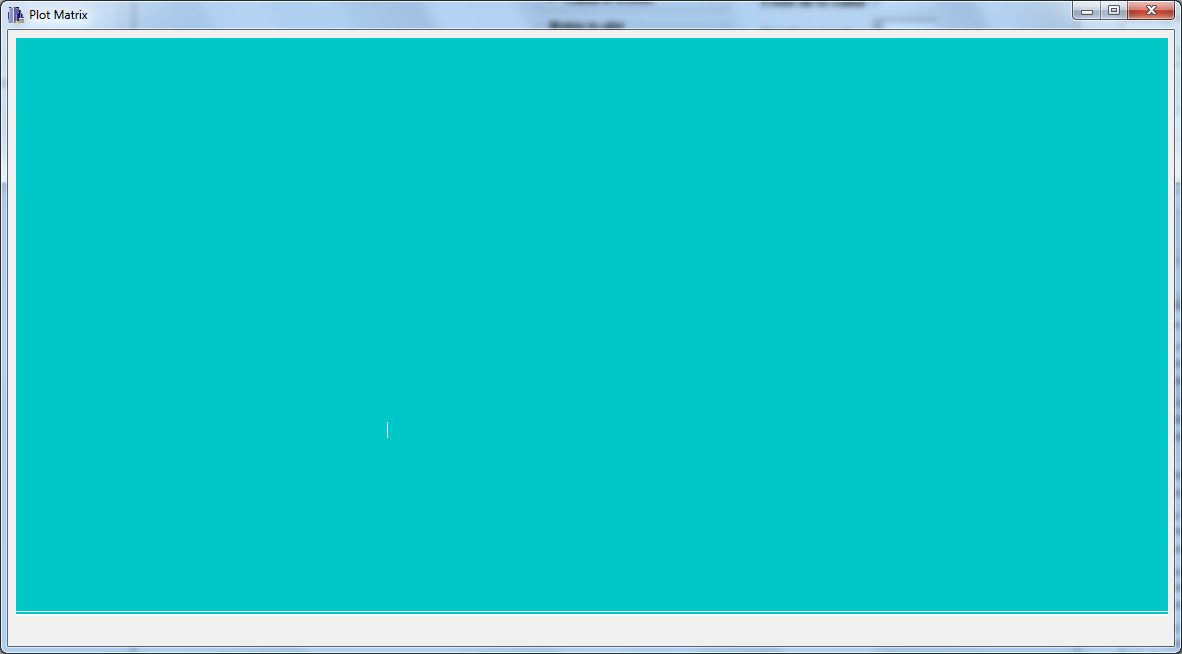
\includegraphics[width = 12cm]{Pictures/Chip6/discri_0.png}
        \label{fig:discri0_chip6}
        \caption{Discriminators output for thresholds set to 0. Few pixels on a column are always closed.}
      \end{center}
    \end{figure}
  
    \item Discriminators calibration:
    \begin{center}
    \begin{tabular}{ M{1.3cm} M{1.3cm} M{1.3cm} M{1.3cm} M{1.3cm} M{1.3cm} M{1.3cm} M{1.3cm} M{1.3cm} }
      \hline %-------------------------------------------------------------------
      \rowcolor{light-gray} $V_{ref1_A}$ START  & $V_{ref1_B}$ START & $V_{ref1_C}$ START & $V_{ref1_D}$ START & $V_{ref2}$ & $V_{ref1_A}$ STOP & Step & Event nb / step & Number of Runs \tabularnewline
      \hline %-------------------------------------------------------------------
      \hline %-------------------------------------------------------------------
      104  &  135  &  119  & 193  &  98  &  160  &  2  &  500  &  29  \tabularnewline
      \hline %-------------------------------------------------------------------
    \end{tabular}
    \end{center}

    \item Temporal noise, fixed pattern noise and offset:

            \begin{center}
              \begin{tabular}{ c c c c }
                \hline %----------------------------
         \rowcolor{light-gray}         Matrix  &  TN   &  FPN  &  Offset  \tabularnewline
                \hline %----------------------------
                \hline %----------------------------
                    A     & 1.023 & 0.574 & 0.412    \tabularnewline
                \hline %----------------------------
                    B     & 0.963 & 0.276 & 0.715   \tabularnewline
                \hline %----------------------------
                    C     & 1.052 & 0.501 & 0.524   \tabularnewline
                \hline %----------------------------
                    D     & 1.056 & 0.479 & 0.457    \tabularnewline
                \hline %----------------------------
              \end{tabular}
            \end{center}

    \item FHR: 
  
    \end{itemize}

    \subsubsection{Chip 5}
  
    Few pixels are stuck to 1 on the sub-matrix C.
  
    \begin{itemize}
  
    \item Estimation of the "middle points":
    \begin{center}
    \begin{tabular}{ c c c c c }
      \hline %-------------------------------------------------------------------------------------
      \rowcolor{light-gray} $V_{ref_2}$  &   $V_{ref_{1A}}$  &   $V_{ref_{1B}}$  &   $V_{ref_{1C}}$  &   $V_{ref_{1D}}$  \tabularnewline
      \hline %-------------------------------------------------------------------------------------
      \hline %-------------------------------------------------------------------------------------
      98        &        177        &         169       &       109         &        67        \tabularnewline
      \hline %-------------------------------------------------------------------------------------
    \end{tabular}
    \end{center}
  
    \item Discriminators calibration:
    \begin{center}
    \begin{tabular}{ M{1.3cm} M{1.3cm} M{1.3cm} M{1.3cm} M{1.3cm} M{1.3cm} M{1.3cm} M{1.3cm} M{1.3cm} }
      \hline %-------------------------------------------------------------------
      \rowcolor{light-gray} $V_{ref1_A}$ START  & $V_{ref1_B}$ START & $V_{ref1_C}$ START & $V_{ref1_D}$ START & $V_{ref2}$ & $V_{ref1_A}$ STOP & Step & Event nb / step & Number of Runs \tabularnewline
      \hline %-------------------------------------------------------------------
      \hline %-------------------------------------------------------------------
      104  &  135  &  119  & 193  &  98  &  160  &  2  &  500  &  29  \tabularnewline
      \hline %-------------------------------------------------------------------
    \end{tabular}
    \end{center}
 
    \item Temporal noise, fixed pattern noise and offset:

            \begin{center}
              \begin{tabular}{ c c c c }
                \hline %----------------------------
         \rowcolor{light-gray}         Matrix  &  TN   &  FPN  &  Offset  \tabularnewline
                \hline %----------------------------
                \hline %----------------------------
                    A     & 0.939 & 0.369 & 0.314    \tabularnewline
                \hline %----------------------------
                    B     & 0.993 & 0.264 & 0.679   \tabularnewline
                \hline %----------------------------
                    C     & 1.010 & 0.385 & 0.407   \tabularnewline
                \hline %----------------------------
                    D     & 1.051 & 0.340 & 0.825    \tabularnewline
                \hline %----------------------------
              \end{tabular}
            \end{center}
    \end{itemize}

   \subsubsection{Chip 4}
  
  
    \begin{itemize}
  
    \item Estimation of the "middle points":
    \begin{center}
    \begin{tabular}{ c c c c c }
      \hline %-------------------------------------------------------------------------------------
      \rowcolor{light-gray} $V_{ref_2}$  &   $V_{ref_{1A}}$  &   $V_{ref_{1B}}$  &   $V_{ref_{1C}}$  &   $V_{ref_{1D}}$  \tabularnewline
      \hline %-------------------------------------------------------------------------------------
      \hline %-------------------------------------------------------------------------------------
      98        &        119        &         121       &       85         &        126       \tabularnewline
      \hline %-------------------------------------------------------------------------------------
    \end{tabular}
    \end{center}
  
    \item Discriminators calibration:
    \begin{center}
    \begin{tabular}{ M{1.3cm} M{1.3cm} M{1.3cm} M{1.3cm} M{1.3cm} M{1.3cm} M{1.3cm} M{1.3cm} M{1.3cm} }
      \hline %-------------------------------------------------------------------
      \rowcolor{light-gray} $V_{ref1_A}$ START  & $V_{ref1_B}$ START & $V_{ref1_C}$ START & $V_{ref1_D}$ START & $V_{ref2}$ & $V_{ref1_A}$ STOP & Step & Event nb / step & Number of Runs \tabularnewline
      \hline %-------------------------------------------------------------------
      \hline %-------------------------------------------------------------------
      91  &  93 & 57  & 98  &  98  &  147  &  2  &  500  &  29  \tabularnewline
      \hline %-------------------------------------------------------------------
    \end{tabular}
    \end{center}
 
    \item Temporal noise, fixed pattern noise and offset:

            \begin{center}
              \begin{tabular}{ c c c c }
                \hline %----------------------------
         \rowcolor{light-gray}         Matrix  &  TN   &  FPN  &  Offset  \tabularnewline
                \hline %----------------------------
                \hline %----------------------------
                    A     & 0.961 & 0.386 & 0.463    \tabularnewline
                \hline %----------------------------
                    B     & 0.945 & 0.235 & 0.513   \tabularnewline
                \hline %----------------------------
                    C     & 1.027 & 0.488 & 0.590   \tabularnewline
                \hline %----------------------------
                    D     & 1.947 & 0.362 & 0.703    \tabularnewline
                \hline %----------------------------
              \end{tabular}
            \end{center}
    \end{itemize}

    \subsubsection{Chip 3}
    
    \begin{itemize}
  
    \item Estimation of the "middle points":
    \begin{center}
    \begin{tabular}{ c c c c c }
      \hline %-------------------------------------------------------------------------------------
      \rowcolor{light-gray} $V_{ref_2}$  &   $V_{ref_{1A}}$  &   $V_{ref_{1B}}$  &   $V_{ref_{1C}}$  &   $V_{ref_{1D}}$  \tabularnewline
      \hline %-------------------------------------------------------------------------------------
      \hline %-------------------------------------------------------------------------------------
      98        &        191        &         145       &       95         &        73        \tabularnewline
      \hline %-------------------------------------------------------------------------------------
    \end{tabular}
    \end{center}
  
    \item Discriminators calibration:
    \begin{center}
    \begin{tabular}{ M{1.3cm} M{1.3cm} M{1.3cm} M{1.3cm} M{1.3cm} M{1.3cm} M{1.3cm} M{1.3cm} M{1.3cm} }
      \hline %-------------------------------------------------------------------
      \rowcolor{light-gray} $V_{ref1_A}$ START  & $V_{ref1_B}$ START & $V_{ref1_C}$ START & $V_{ref1_D}$ START & $V_{ref2}$ & $V_{ref1_A}$ STOP & Step & Event nb / step & Number of Runs \tabularnewline
      \hline %-------------------------------------------------------------------
      \hline %-------------------------------------------------------------------
      163  &  117  &  65  & 45  &  98  &  219  &  2  &  500  &  29  \tabularnewline
      \hline %-------------------------------------------------------------------
    \end{tabular}
    \end{center}
 
    \item Temporal noise, fixed pattern noise and offset:

            \begin{center}
              \begin{tabular}{ c c c c }
                \hline %----------------------------
         \rowcolor{light-gray}         Matrix  &  TN   &  FPN  &  Offset  \tabularnewline
                \hline %----------------------------
                \hline %----------------------------
                    A     & 0.987 & 0.450 & -0.035    \tabularnewline
                \hline %----------------------------
                    B     & 0.957 & 0.289 & 0.126   \tabularnewline
                \hline %----------------------------
                    C     & 1.044 & 0.521 & 0.224   \tabularnewline
                \hline %----------------------------
                    D     & 1.065 & 0.435 & -0.006    \tabularnewline
                \hline %----------------------------
              \end{tabular}
            \end{center}
    \end{itemize}

    \subsubsection{2}

    The chip was disconnected from the flex.

    \subsubsection{1}

    The chip is still connected to the flex but is not working properly. In the JTAG files, the discriminators are set to 225.

    \begin{figure}[!h]
      \begin{center}
        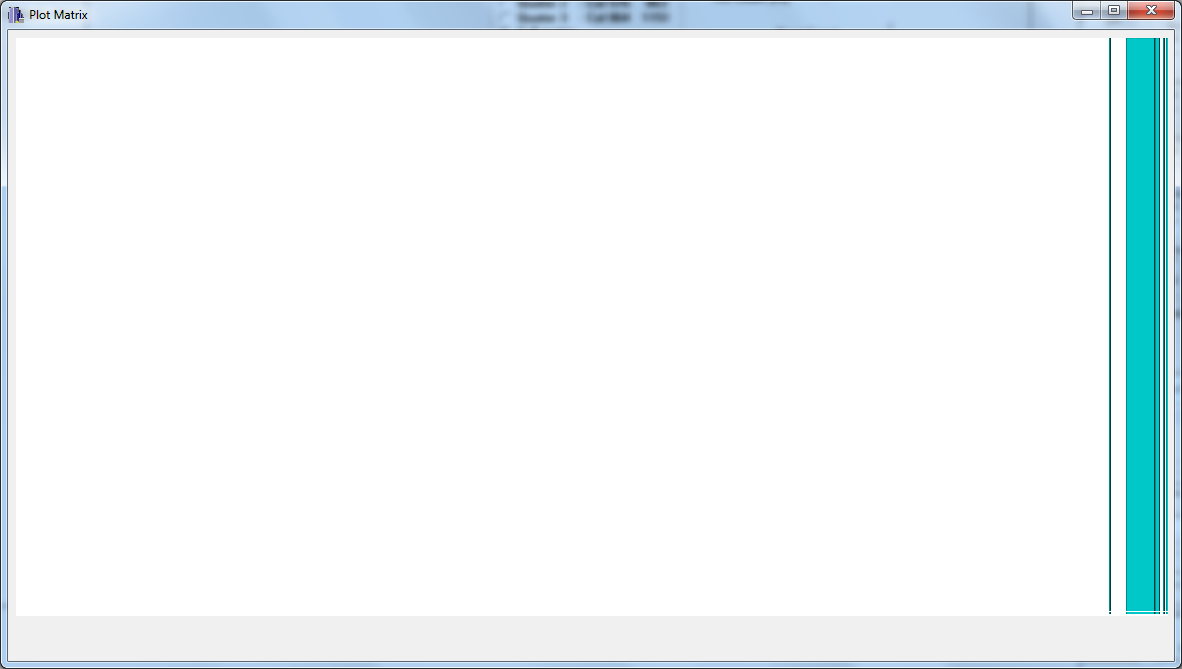
\includegraphics[width = 12cm]{Pictures/Chip1/discri_0.png}
        \label{fig:discri0_chip1}
        \caption{Discriminators output for thresholds set to 0. Almost all of the discriminators are always closed.}
      \end{center}
    \end{figure}

  \section{Fake Hit Rate}
\end{document}
